\textbf{COLUNI 2023 -- Questão 24}\par\medskip Em uma aula de Laboratório de Física, o objetivo dos estudantes era obter, graficamente, o valor em Ohms (Ω) da resistência de dois resistores ôhmicos $R_1$ e $R_2$. Para cada um dos resistores foi montado um circuito elétrico simples, composto por uma fonte de tensão contínua e variável, um voltímetro, para medir a diferença de potencial nos resistores, ou seja, a Voltagem; e um amperímetro, para medir a corrente elétrica no circuito. Para cada diferença de potencial aplicada no circuito, por meio da fonte de tensão, foram anotados nos resistores, de forma independente, os valores das diferenças de potenciais e correntes fornecidos pelos voltímetro e amperímetro, respectivamente. Com os conjuntos de dados obtidos foi possível construir o gráfico a seguir:

% COLUNI-AUTO-FIGURES-BEGIN
\begin{figure}[htbp]
\centering
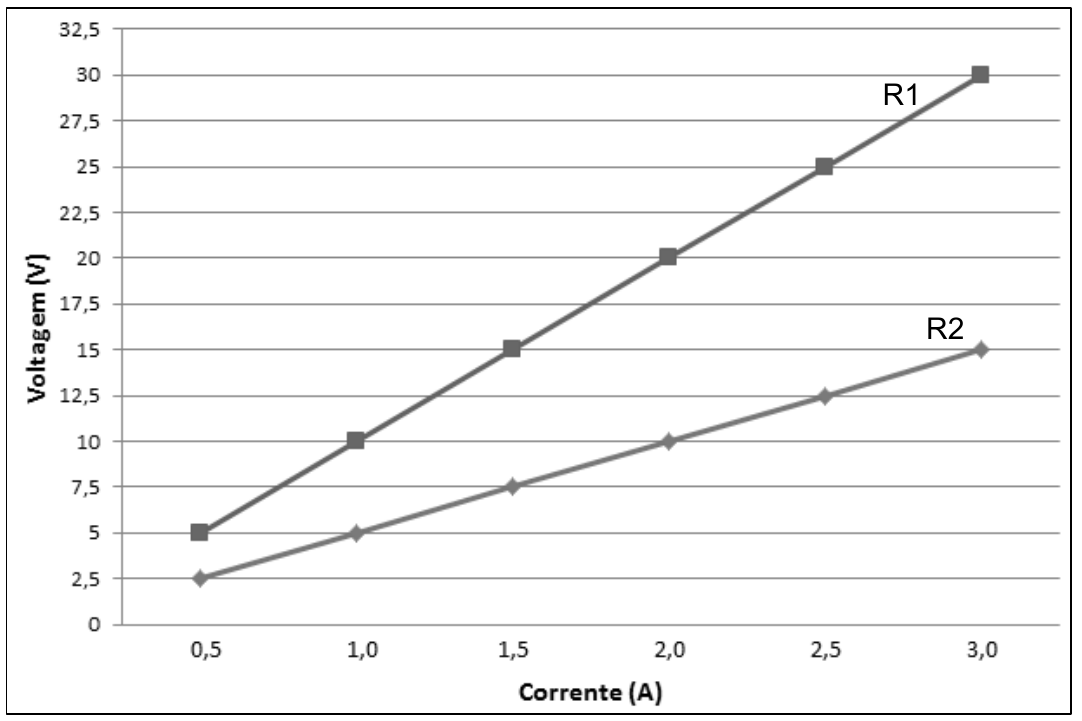
\includegraphics[width=0.95\linewidth]{static/simulados/coluni/figuras/2023/questao-24/figura-1.png}
\end{figure}
% COLUNI-AUTO-FIGURES-END
Considerando as informações do gráfico, é INCORRETO afirmar:
\begin{enumerate}
\item O valor da resistência de ambos os resistores, $R_1$ e $R_2$, permanece constante.
\item O valor da resistência $R_2$ em Ohms (Ω) é menor do que o valor da resistência $R_1$ em Ohms (Ω).
\item Na corrente de 1,0 A, a diferença de potencial aplicada em $R_1$ é o dobro da aplicada em R2.
\item O valor da resistência $R_1$ em Ohms (Ω) é a metade do valor da resistência $R_2$ em Ohms.\end{enumerate}
